\documentclass[tikz]{standalone}
\usepackage[utf8x]{inputenc}
\usepackage{tikz}
\begin{document}
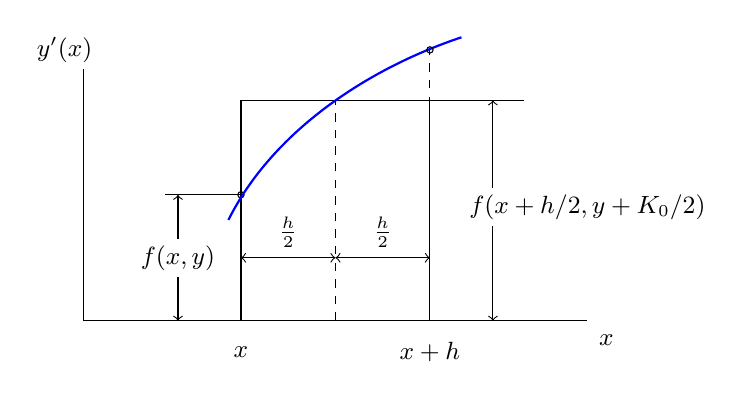
\begin{tikzpicture}[scale=0.8, font=\small]
    \draw (0,0) -- (8,0);
    \draw (0,0) -- (0,4);
    \draw (-0.3,4.3) node {$y^{\prime}(x)$};
    \draw (8.3,-0.3) node {$x$};
    \draw (2.5,0) rectangle (5.5,3.5);
    \draw (2.5,-0.5) node {$x$};
    \draw (5.5,-0.5) node {$x + h$};
    \draw (1.5,1) node {$f(x, y)$};
    \draw (2.5,2) circle (0.05);
    \draw (2.5,2) -- (1.3,2);
    \draw [->] (1.5,1.3) -- (1.5,2);
    \draw [->] (1.5,0.7) -- (1.5,0);
    \draw [blue, thick](2.3,1.6) .. controls(3,3) and (4.5,4) .. (6,4.5);
    \draw [dashed] (5.5,0) -- (5.5,4.3);
    \draw (5.5,4.3) circle (0.05);
    \draw [dashed] (4,0) -- (4,3.5);
    \draw [<->] (2.5,1) --  node [above=0.2] {$\frac{h}{2}$}(4,1);
    \draw [<->] (4,1) --  node [above=0.2] {$\frac{h}{2}$}(5.5,1);
    \draw (5.5,3.5) -- (7,3.5);
    \draw (8,1.8) node {$f(x + h/2, y + K_{0}/2)$};
    \draw [->] (6.5,2.1) -- (6.5,3.5);
    \draw [->] (6.5,1.5) -- (6.5,0);    
\end{tikzpicture}

\end{document}